%
% $Id: $
%
%
% Compilar a .pdf con LaTeX (pdflatex)
% Es necesario instalar Beamer (paquete latex-beamer en Debian)
%

%
% Gr�ficos:
% Los gr�ficos pueden suministrarse en PNG, JPG, TIF, PDF, MPS
% Los EPS deben convertirse a PDF (usar epstopdf)
%

\documentclass{beamer}
\usetheme{GSyC}
%\usebackgroundtemplate{\includegraphics[width=\paperwidth]{format/libresoft-bg.png}}
%\usepackage[spanish]{babel}
\usepackage[latin1]{inputenc}
\usepackage{graphics}
\usepackage{amssymb} % Simbolos matematicos

\ProcessOptions

%% Metadatos del PDF.
\hypersetup{
  pdftitle={Protocolos para la Transmisi�n de Audio y V�deo por Internet},
  pdfauthor={Gregorio Robles, Jes�s M. Gonz�lez Barahona},
  pdfcreator={GSyC, Universidad Rey Juan Carlos},
  pdfproducer=PDFLaTeX,
  pdfsubject={Protocolos para la Transmisi�n de Audio y V�deo por Internet},
}
%%

\begin{document}

\title{�C�mo conseguir un buen trabajo (tecnol�gico)?}
\subtitle{Protocolos para la Transmisi�n de Audio y V�deo en Internet}
\institute{\{grex,jgb\}@gsyc.urjc.es \\
GSyC, Universidad Rey Juan Carlos}
\author[Gregorio Robles, Jes�s M. Gonz�lez Barahona]{Gregorio Robles, Jes�s M. Gonz�lez Barahona}
\date[Nov 2014]{12 de noviembre de 2014}


\frame{
\maketitle
}


% Si el titulo o el autor se quieren acortar para los pies de p�gina
% se pueden redefinir aqu�:
%\title{Titulo corto}
%\author{Autores abreviado}


%% LICENCIA DE REDISTRIBUCION DE LAS TRANSPAS
\frame{
~
\vspace{4cm}

\begin{flushright}

\includegraphics[width=2.2cm]{figs/by-sa}

{\tiny
(cc) 2014 Gregorio Robles, Jes�s M. Gonz�lez Barahona \\
  Some rights reserved. This work licensed under Creative Commons \\
  Attribution-ShareAlike License. To view a copy of full license, see \\
\ \\
  http://creativecommons.org/licenses/by-sa/3.0/ or write to \\
  Creative Commons, 559 Nathan Abbott Way, Stanford, \\
  California 94305, USA. \\
\ 
}
\end{flushright}
}
%%

%-----------------------    ---------------------------------

\begin{frame}
\frametitle{�Qu� es un trabajo \emph{bueno}?}

\begin{itemize}
   \item Un trabajo que te permita ser creativo
   \item Un trabajo donde trabajes con �ltimas tecnolog�as
   \item Un trabajo donde puedas ascender sin dejar de ser ingeniero
   \item Un trabajo donde te paguen bien (y otros beneficios)
\end{itemize}

Hay muchas empresas donde buscan este tipo de perfil: Google, Apple, Facebook,
Microsoft, Yahoo!, Amazon...

\end{frame}

%-----------------------    ---------------------------------

\begin{frame}
\frametitle{Salarios en las compa��as top}

\begin{center}
  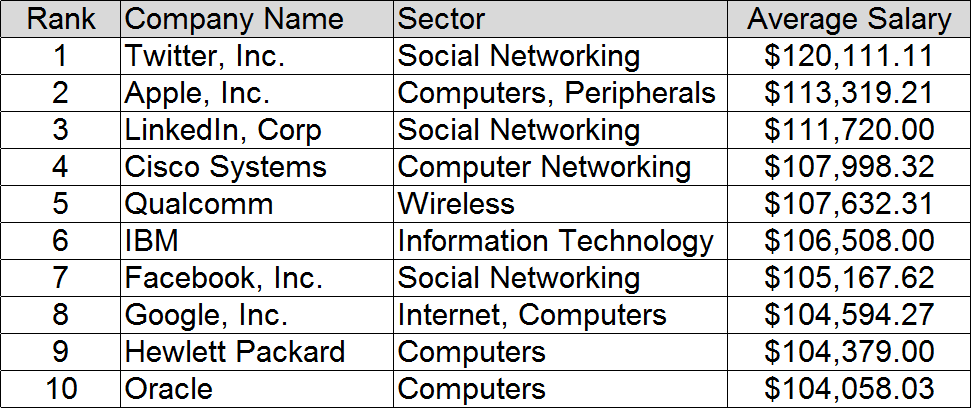
\includegraphics[width=10cm]{figs/toppaytech.png}
\end{center}


\begin{flushright}
{\tiny
http://img59.imageshack.us/img59/802/toppaytech.png
}
\end{flushright}

\end{frame}


%-----------------------    ---------------------------------

\begin{frame}
\frametitle{�Qu� te piden en estos trabajos?}

\begin{itemize}
   \item Estructuras de datos
   \item Algoritmia
   \item Experiencia en programaci�n
   \item Redes de ordenadores
   \item Sistemas operativos
\end{itemize}

\end{frame}


%-----------------------    ---------------------------------

\begin{frame}
\frametitle{M�s lecturas}

\begin{itemize}
   \item Hay varios libros sobre este tema, algunos en la biblioteca:
   \begin{itemize}
     \item Cracking the coding interview: 150 programming interview questions and solutions
     \item The Google Interview
     \item Elements of Programming Interviews: The Insiders' Guide
     \item Top 10 coding interview problems asked in Google with solutions: Algorithmic Approach
     \item Are You Smart Enough to Work at Google?: Fiendish Puzzles And Impossible Interview Questions From The World's Top Companies
     \item Get a Job WITHOUT an Interview - Google \& Beyond!: ``We don't mind to lose a good applicant, but definitely not hire a bad applicant.''
     \item The Google Resume: How to Prepare for a Career and Land a Job at Apple, Microsoft, Google, or any Top Tech Company
   \end{itemize}
\end{itemize}

\end{frame}



\frame{
\maketitle
}

\end{document}
